\section{System Design}

Draw the runtime on a napkin and it is linear: telemetry in, policy guesses, maybe the gate vetoes, the shield always edits last, actuators see something bounded. Chain commits ride afterward if you want receipts two companies can argue over later.

\[
\text{state telemetry} \rightarrow \text{policy proposal} \rightarrow \text{uncertainty gate} \rightarrow \text{shield} \rightarrow \text{executed action}.
\]

Learning stays in Python/Sim; hashes land once the action is final so nobody pretends the ledger is on the hot gradient path.

\subsection{System Diagram}

\begin{figure}[H]
\centering
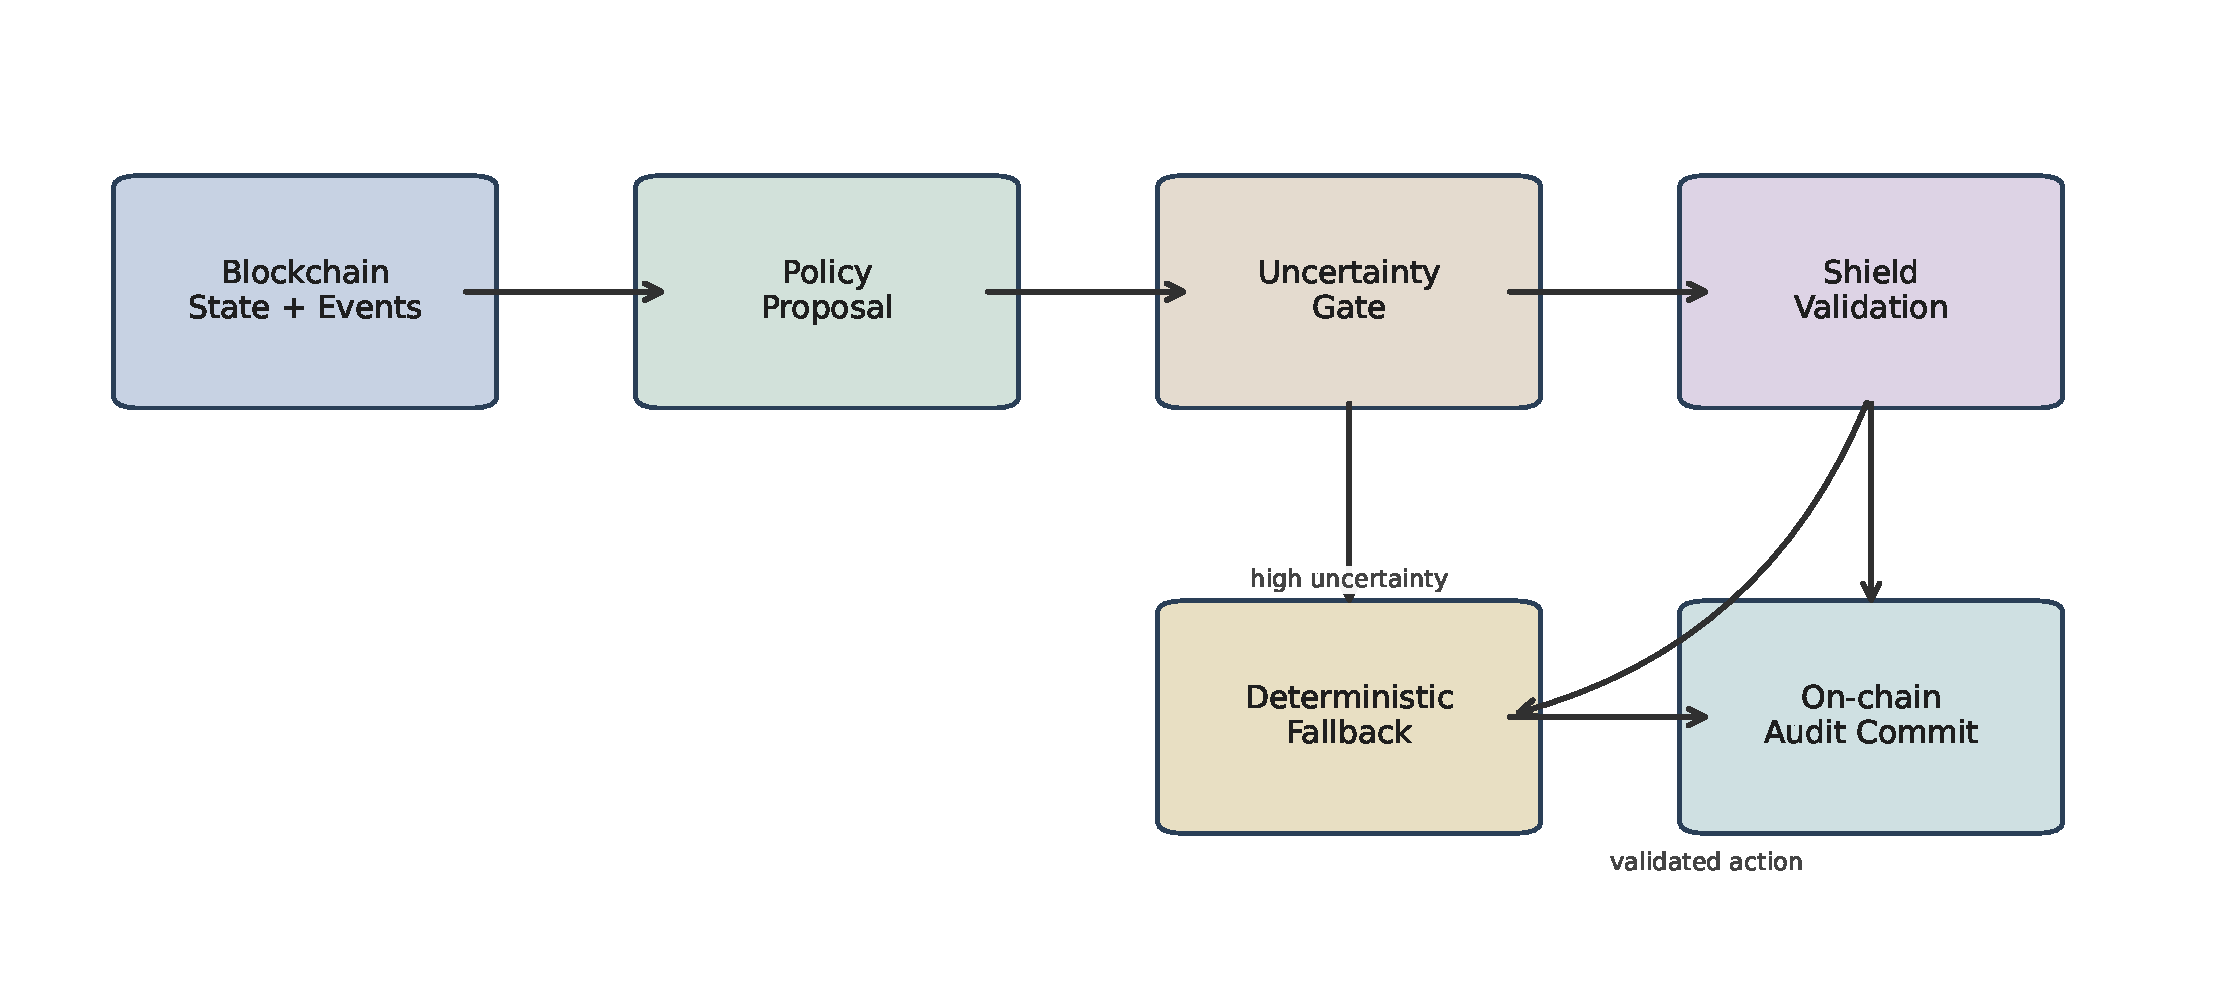
\includegraphics[width=0.95\linewidth]{figures/architecture_flow.pdf}
\caption{Runtime sketch: policy, gate, shield, optional commit.}
\label{fig:system-mermaid-rendered}
\end{figure}

\subsection{Data and Control Flow}

Peers and txs move ledger state through RPC plus validation. The controller ingests a compressed governance vector and proposes bounded knobs---difficulty, block size, gas limit. Same story as the napkin, typeset with the shield explicit:

\begin{equation}
\begin{aligned}
\text{State telemetry} &\rightarrow \text{policy proposal} \rightarrow \text{uncertainty gate} \\
&\rightarrow \text{safety shield} \rightarrow \text{on-chain commit}.
\end{aligned}
\end{equation}

Gate can punt to a heuristic first; shield can clamp or reject anyway. Every number in the paper assumes that gated-then-shielded path. Receipt/Merkle minutiae sit in appendix text if you need them.

\subsection{API Contracts}

RPC structs are typed; junk input throws instead of silently widening what the adaptive layer may try. Negative-path tests on malformed fields are boring and necessary.

\subsection{Operational Guardrails}

Typed interfaces, those tests, and a fixed ordering between policy, gate, and shield keep multi-node runs from decaying into ``works on my laptop.'' Zero novelty medals; it is what keeps pages legible when pagerduty fires at 2\,am.
